\documentclass[11pt]{article}
\renewcommand{\baselinestretch}{1.20} 
\usepackage[utf8]{inputenc}
\usepackage[english]{babel}
\usepackage{graphicx}
\usepackage{wrapfig}
\usepackage{subcaption}
\usepackage{geometry}
\usepackage{xcolor}
\usepackage{float}
\usepackage{mdframed}
\usepackage{fancyhdr}
\usepackage{lastpage}
\usepackage{booktabs}% http://ctan.org/pkg/booktabs
\newcommand{\tabitem}{~~\llap{\textbullet}~~}
\geometry{a4paper, total={170mm,237mm}, left=20mm, top=20mm}
\setlength{\abovecaptionskip}{15pt plus 3pt minus 2pt}

\pagestyle{fancy}
\fancyhf{}
\rfoot{Side \thepage \hspace{1pt} / \pageref{LastPage}}
\begin{document}
    
    % Title page
    \begin{titlepage}
    \centering
	
\includegraphics[width=0.35\textwidth]{Projectdoc/Assets/Illustrationer/aau_logo_en.pdf}\par\vspace{1cm}
	{\scshape\Large Struktureret System Udvikling\par}
	\vspace{0.2cm}
	{\huge\bfseries Workshop 3\par}
	\vspace{0.2cm}
	{\scshape\Large ITC - B125\par}
	\vspace{2cm}
	{\Large\itshape 
    	Mikkel Steen Hansen\\
        Benjamin Bach Jensen\\
        Daniel Vestergaard Jensen\\
    \par}
	\vfill
	\vfill
\end{titlepage}
    
    % Table of contents
    \renewcommand{\baselinestretch}{0.8}
    \tableofcontents
    \renewcommand{\baselinestretch}{1.20}
    \newpage
    
    \section{Beskrivelse}
    \textbf{Mini projekt: Vejr station}\\
    Dagens workshop omhandler at videre udvikle på sidste workshops vejr station, for anvendelse i et parcel hus. I dette workshop ligger fokus i testing og error handling.\\
    Tanken bag projektet er at forskellige sensorer registrerer en eller flere informationer der skal til for at beskrive vejret. Disse data samles op via en enhed der kan videregive information til en app på brugerens smartphone eller computer, evt. krydret med en præcis vejrudsigt i den kommende time ved at udnytte services fra DMI
    eller anden vejr tjeneste.
    
    \begin{figure}[H]
        \centering
        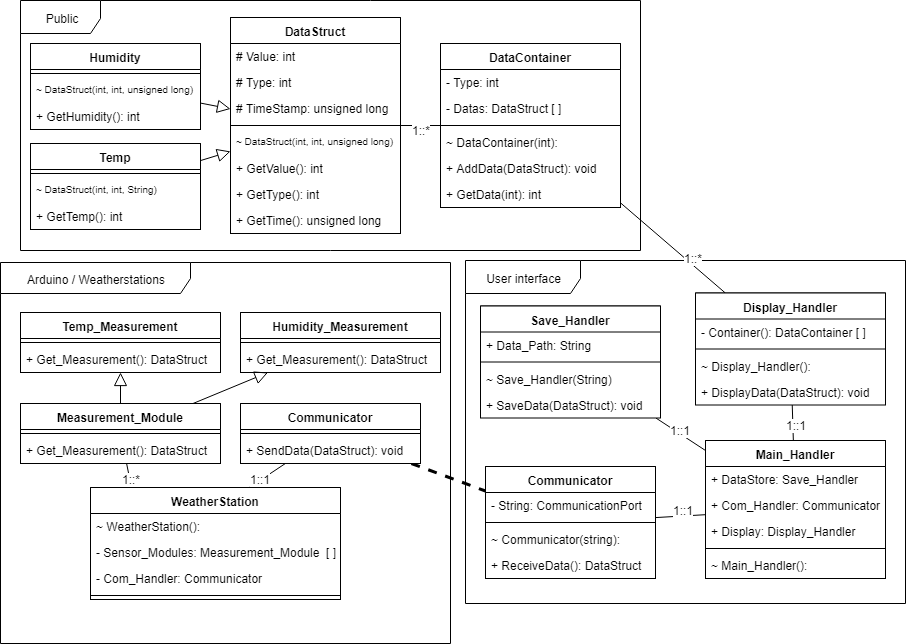
\includegraphics[width=1\textwidth,angle=0]{Struktureret_System_Udvikling/Workshop_2/Assets/Workshop2_ClassDiagram.png}
        \caption{Interaction Class Diagram}
        \label{fig:ClassDiagram}
    \end{figure}
    \noindent
    Gruppen har i dette workshop valgt at lægge mest vægt på testing og handling i koden omhandlende Userinterface. Hvor her referere til sidste workshops class diagram \ref{fig:ClassDiagram}.
    Dog forefindes stadig mindre whiteboxtesting path tests på Verstationens side. F.eks. kan man under Temp\_Measurement og Humidity\_Measurement findes følgende, der tester ikke kun tester den litererede path men også en minour result test.
    
    \begin{figure}[H]
        \begin{subfigure}{0.3\textwidth}
            \centering
            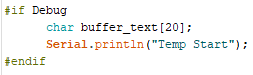
\includegraphics[width=1\linewidth, height=2cm]{Struktureret_System_Udvikling/Workshop_3/Assets/Start.PNG}
            \caption{Path testing}
            \label{fig:TestPath}
        \end{subfigure}
        \begin{subfigure}{0.7\textwidth}
            \centering
            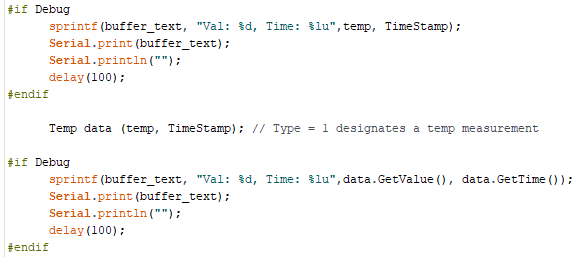
\includegraphics[width=1\linewidth, height=7cm]{Struktureret_System_Udvikling/Workshop_3/Assets/Secound.PNG}
            \caption{Minour result testing}
            \label{fig:TestRes}
        \end{subfigure}
        \label{fig:Testing}
    \end{figure}
    
    %Den anden side... pc
    
    \noindent
    Foruden førnævnte har gruppen også inplamenteret følgende funktionaliteter:
    SquareRoot og BubbleSort.
    Dog da disse funktionaliteter har påvist manglende test, samt ikke udgiver det forventede resultat har vi også gennem gået en retning af disse ved anvendelse af whitebox testing, en testings metode, hvor funktionaliteten gennemgåes først i en flowgraf ved dens forventede udputs for forudbestemte muligheder eller inputs, og dernest også ved nærmere inspektion af selve koden, samt dens faktiske givende resultater.
    
    \noindent
    For SquareRoot har gruppen dannet følgende Flowgraf:\\
    \begin{subfigure}{1\textwidth}
        \centering
        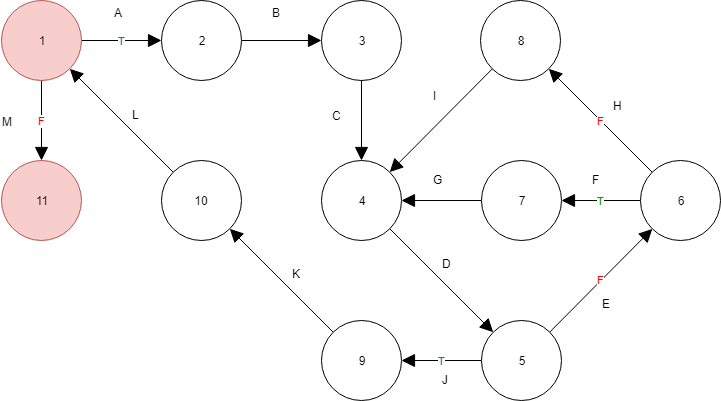
\includegraphics[width=0.8\linewidth, height=6cm]{Struktureret_System_Udvikling/Workshop_3/SquareRoot_FlowGraph.png}
        \caption{BoobleSort Flowgraph}
        \label{fig:BoobleSortGraph}
    \end{subfigure}
    Og kan derfor, ved et retmessigt forløb forvente en gennemgang i vejene:\\
    A-B-\{C-D-E-[F-G/H-I]\}*"Nødvendige gæt"-C-D-J-K-L-M\\
    Hvor \{ - \} definere et loop af en vis størelse, der altid skal opfylde det beskrævende mønster.\\
    Eneste undvigelse kan ses ved F-G der også kan være beskrevet ved vejen H-I.\\
    \\
    Efter første gennemgang kan dog konkluderes at funktionen tager følgende vej:\\
    A-B-C-D-E-F-G-D-E-F-G-D-E-F-.....
    
    \begin{subfigure}{1\textwidth}
        \centering
        \includegraphics[width=1\linewidth, height=7cm]{Struktureret_System_Udvikling/Workshop_3/}
        \caption{BoobleSort Flowgraph}
        \label{fig:BoobleSortGraph}
    \end{subfigure}
    
    \\
    \noindent
    For BubbleSort har gruppen dannet følgende Flowgraf:\\
    \begin{subfigure}{1\textwidth}
        \centering
        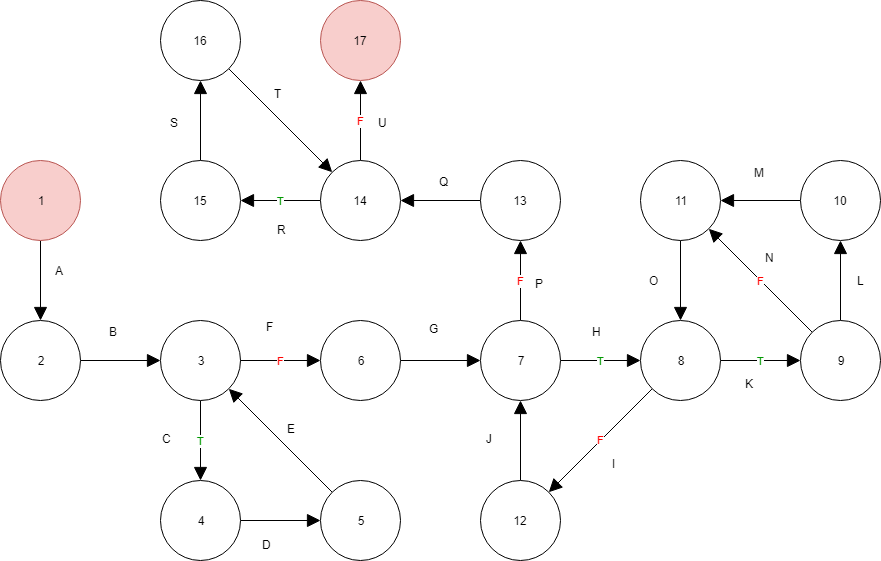
\includegraphics[width=1\linewidth, height=7cm]{Struktureret_System_Udvikling/Workshop_3/Booble_Sort_Flowgraph.png}
        \caption{BoobleSort Flowgraph}
        \label{fig:BoobleSortGraph}
    \end{subfigure}
    Og kan derfor, ved et retmessigt forløb forvente en gennemgang i vejene:\\
    A-B-\{C-D-E\}*"Array størelse"-F-G-\{H-\{K-[N/L-M]-O\}-I-J\}-P-O-\{R-S-T\}*"Array størelse"-U\\
    Hvor \{ - \} definere et loop af en vis størelse, der altid skal opfylde det beskrævende mønster.\\
    Eneste undvigelse kan ses ved N der også kan være beskrevet ved vejen L-M.\\
    \\
    Efter første gennemgang kan dog konkluderes at funktionen tager følgende vej:\\
    A-B-\{C-D-E\}*4-F-G-H-K-K-K-K-......\\
    Derved kan ses at her forekommer 2 typer af fejl:\\
    Første i loopet mellem C,D,E der ikke fuldender den forvendtede længte. Denne kan løses ved kodens forloop der skal rettes fra "for(int i = 0; i \textless --size; i++)" til "for(int i = 0; i \textless= size; i++)".\\
    Anden fejl forekommer i loopet ved K, hvor man ved en nærmere kode inspektion kan se at de omkringliggende loops mangler afsluttende brakkets.\\
    Efter anden gennemgang kan dog stadig ses, at funktionen ikke tager forventede vej, da næste forventede vej ville være: F-G-H-K-L-M-O-K-L-M-O..., for det diffenerede array "10-2-5...", og ikke den resulterende vej: F-G-H-K-N-O-K-N-O...\\
    Denne fejl skal findes i sorterings kodens tjek for, om et ellement på den givende possition er stører end næsteværende ellement. Koden "if(a[j] \textless a[i+1])" skal derfor rettes til "if(a[j] \textgreater a[j+1])", da j diffinerer nuværende tjek og i diffinerer arrayets gennemgang. Efterfølgende skal dog også bemærkes at det samme deffinerede "i", også anvendt i koden "hold = a[i];", heller ikke relatere til den forvendtede possition, og skal derfor af samme grunde rettes til "hold = a[j];".\\
    Efter sidste gennemgangs rettelser, kan sidste fejlrettelse findes i loopet diffineret fra H-J, der ved et gennemløb bliver affsluttet inden dens forvendtede ressultat. Altså kan fejlen findes i koden "for(i = 0; i \textless (size \&\& switched); i++)", hvor her bemærkes at loopets header indeholder en forkert sat ramme "i \textless (size \&\& switched)" skal derfor rettes til "(i \textless size) \&\& switched".

    \noindent
    Disse funktionaliterer er efterfølgende blevet anvendt i følgende støre fonktionaliteter:
    Gennemsnit og standardafvigelsesberegningsfunktionalitet,
    samt Sorterings alguritme.
    Til disse har gruppen også efterfølgende anvendt Blackbox testing, en metode hvor forventede output sammenligenes med faktuelle resultat, uden brug af kode inspektion, for både førnævnte induviduelle funktionaliteter såvel som hele systeme, til efterfølgende kontrol tests.
    
\end{document}